\subsection{Raggi cosmici al livello del suolo}  % titolo provvisorio

I raggi cosmici primari sono particelle accelerate da sorgenti astrofisiche che colpiscono continuamente l'atmosfera terrestre. Interagendo con i nuclei in alta atmosfera producono flussi di particelle secondarie che a loro volta interagiscono o decadono provocando sciami di particelle.

Al livello del suolo i raggi cosmici carichi sono costituiti principalmente da muoni
e in minor parte da elettroni (e positroni),
come mostrato in Figura~\ref{fig:vertical_angular}\subref{fig:vertical_flux},
dove è riportato il flusso verticale integrato ad una latitudine geomagnetica di $\sim \SI{40}{\degree}$ in funzione della loro energia cinetica. Dal grafico è anche possibile notare come i muoni in arrivo abbiano in pratica tutti energia $>\SI{500}{\MeV}$ e siano perciò considerabili MIP.

\begin{figure}[H]
	\begin{subfigure}[t]{0.48\textwidth}
		\centering
		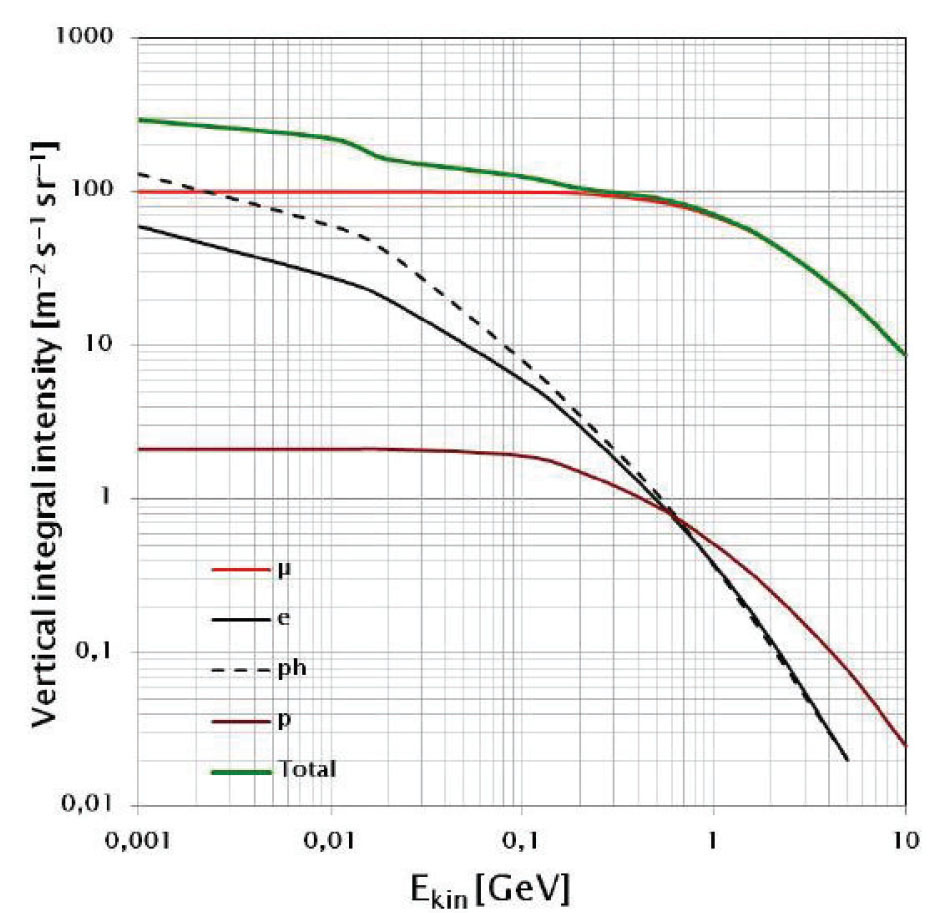
\includegraphics[width=\textwidth]{vertical_flux}
		\caption{\label{fig:vertical_flux}
		Flusso verticale integrato dei raggi cosmici (per ciascuna componente)
		mediato su un ciclo solare di 11 anni al livello del mare
		ad una latitudine geomagnetica di $\sim \SI{40}{\degree}$ in funzione dell'energia cinetica.}
	\end{subfigure}
	\hfill
	\begin{subfigure}[t]{0.48\textwidth}
		\centering
		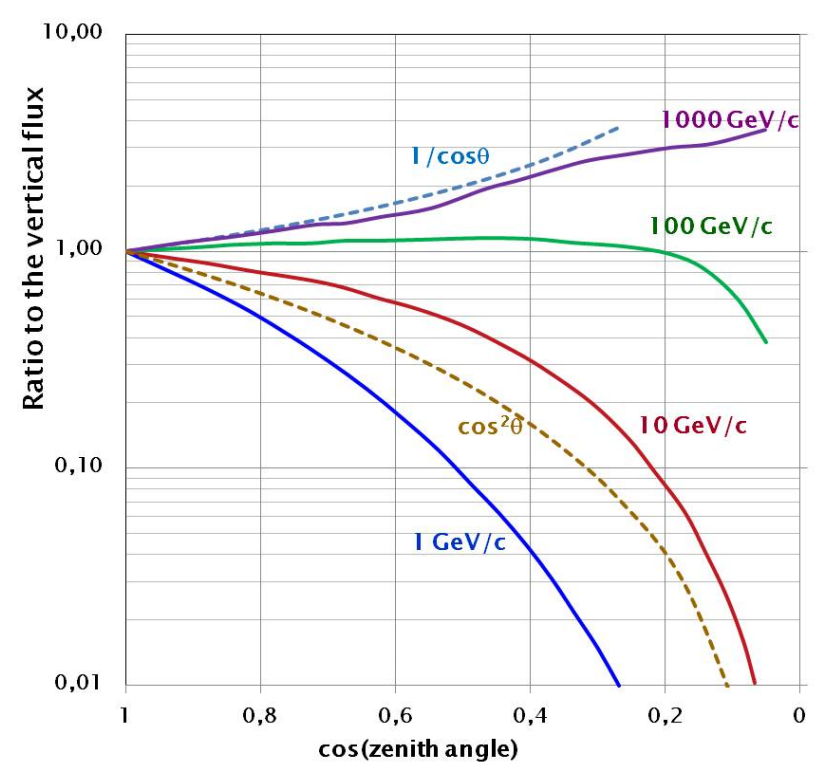
\includegraphics[width=\textwidth]{angular_distribution}
		\caption{\label{fig:angular_distribution}
		Distribuzione angolare dei muoni in funzione dell'impulso
		(distribuzione nell'angolo solido).}
	\end{subfigure}
	\caption{\label{fig:vertical_angular}
	Proprietà dei raggi cosmici al livello del suolo, fonte \cite{1}.}
\end{figure}

Il flusso verticale di muoni con energia $E_{\mu} > \SI{1}{\GeV}$ attraverso una superficie orizzontale vale $I_v(E_{\mu} > \SI{1}{\GeV}) \sim \SI{70}{m^{-2} s^{-1} sr^{-1}}$ che corrisponde alla nota stima di una particella per $\SI{}{cm^2}$ per minuto. Se scegliamo un taglio in energia meno rigido, più vicino alle condizioni del nostro esperimento (in cui in pratica il taglio in energia è fatto dal soffitto del laboratorio) otteniamo un flusso $I_v(E_{\mu} > \SI{300}{\MeV}) \sim \SI{100}{m^{-2} s^{-1} sr^{-1}}$.

\paragraph{Distribuzione angolare}

La distribuzione angolare del flusso di muoni in arrivo al livello del mare dipende dall'energia degli stessi come mostrato in Figura~\ref{fig:vertical_angular}\subref{fig:angular_distribution}, questo perché muoni più energetici hanno una vita media più lunga e riescono a viaggiare per distanze maggiori prima di decadere.
La Figura~\ref{fig:vertical_angular}\subref{fig:angular_distribution} mostra che per muoni con impulsi dell'ordine di qualche GeV/c la dipendenza del flusso dall'angolo è $\propto \cos^n\theta$ con $n$ intorno a 2.

La distribuzione angolare del flusso di muoni riveste un ruolo importante nella nostra misura poiché l'apparato non può essere ruotato e gli angoli accettati dipendono dalla geometria dell'apparato. Questo vuol dire che senza conoscere la distribuzione angolare dei raggi in arrivo non ci è possibile ottenere il flusso totale (integrato su tutto l'angolo solido) dei muoni in arrivo. Sapendo che la distribuzione dei muoni è approssimabile con $A_0 \cos^n\theta$ e misurando il flusso con accettanze angolari diverse ci è possibile ricavare sia $A_0$ (il flusso verticale) che $n$.

\paragraph{Risultati precedenti in letteratura}

Il flusso di raggi cosmici, oltre a dipendere dal'altitudine, dipende anche dalla latitudine geomagnetica e varia nel tempo seguendo i cicli solari. Questo rende difficile confrontare misure fatte in luoghi e momenti diversi che quindi hanno una certa variabilità.
In \autoref{tab:letteratura} riportiamo un breve elenco di risultati presenti in letteratura. Nella tabella 3.23 in \cite{7}  è riportato un vasto insieme di misure di flussi verticali integrati di raggi cosmici al livello del mare.


\begin{table}
	\small
	\hspace{-3em}
	\begin{tabular}{lccccc}
		\hline
		Autori & Lat. [$\SI{}{\degree N}$]& Alt. [$\SI{}{m}$]& Impulso [$\SI{}{Gev/c}$] &$n$ & \makecell{Flusso a $\theta=0$\\{}[$\times 10^{-3}\si{cm^{-2}s^{-1}sr^{-1}}$]}\\
		\hline
		Crookes, Rastin \cite{2} & 53 & 40 &$\ge$ 0.35 &2.16 $\pm$ 0.01 &9.13  $\pm$ 0.12\\
		Greisen \cite{3} \cite{4}& 54 & 259 &$\ge$ 0.33& 2.1 &8.2  $\pm$ 0.1\\
		Judge, Nash \cite{5}& 53 & s.l.m. & $\ge$ 0.7 & 1.96  $\pm$ 0.22 & --\\
		Fukui et al. \cite{6}& 24 & s.l.m.& $\ge$ 0.34 &-- &7.35 $\pm$ 0.2\\
		Gokhale \cite{7}& 19 & 124 &$\ge$ 0.27 &-- &7.55 $\pm$ 0.1\\
		Karmakar et al. \cite{8}& 16 & 122 &$\ge$ 0.353 &2.2 &8.99 $\pm$ 0.05\\
		Sinha, Basu \cite{9}& 12 & 30 &$\ge$ 0.27 &-- &7.3 $\pm$ 0.2\\
		S. Pal \cite{10}& 10.61 & s.l.m. &$\ge$ 0.280 &2.15 $\pm$ 0.01 &6.217 $\pm$ 0.005\\
		Allkofer et al. \cite{11}& 9 & s.l.m. &$\ge$ 0.32 &-- &7.25 $\pm$ 0.1\\
		S. Pethuraja et al. \cite{12}&1.44 & 160 &$\ge$ 0.11 &2.00 $\pm$ 0.18 & 7.0 $\pm$ 0.5\\
		\hline
	\end{tabular}
	\caption{\label{tab:letteratura}
	Misure in letteratura del flusso verticale e della distribuzione angolare di muoni
	a varie latitudini e altitudini.}
\end{table}

\subsubsection{Selezione in impulso}

Stimiamo l'effetto del tetto sulle particelle in arrivo.
In base alla Figura~\ref{fig:vertical_angular}\subref{fig:vertical_flux},
ci concentriamo su muoni ed elettroni.

\paragraph{Muoni}

Per i calcoli sui muoni ci avvaliamo del noto grafico%
\footnote{\emph{Particle Physics Booklet 2014}, pag. 255}
che mostra il rapporto tra percorso residuo e massa della particella in funzione dell'impulso.
Il rapporto percorso residuo/massa corrispondente a muoni di \SI{300}{MeV}
nel piombo è circa \SI{2e3}{g\,cm^{-2}\,GeV^{-1}}.
Per trovare il percorso residuo bisogna moltiplicare questa quantità per la massa della particella
e dividere per la densità del materiale.
Risulta un percorso residuo di \SI{20}{cm}.
Stimiamo che il tetto equivalga a meno di \SI{20}{cm} di piombo,
quindi anche i muoni cosmici meno energetici non vengono fermati.

\paragraph{Elettroni}

La perdita di energia al minimo di ionizzazione è circa \SI{1.5}{MeV\,g^{-1}\,cm^2}.
Quindi, supponendo un soffitto spesso circa \SI{10}{cm} e densità circa \SI{5}{g\,cm^{-3}},
gli elettroni perdono almeno \SI{70}{MeV}.
Guardando Figura~\ref{fig:vertical_angular}\subref{fig:vertical_flux},
vediamo che allora il flusso verticale di elettroni è meno dell'\SI{8}\% di quello dei muoni.
